\clearpage
\begin{examplebox}
\textbf{例1（母题：标准方程直接求焦半径）。}

已知
\[
E:\ \frac{x^2}{16}+\frac{y^2}{12}=1,\qquad
H:\ x^2-\frac{y^2}{3}=1.
\]
$P$ 是两条曲线第一象限的公共点。求 $PF_1$、$PF_2$。

\begin{center}
% C093: a=4, A=1, c=2; E: x^2/16+y^2/12=1, H: x^2-y^2/3=1
% Intersection P=(2,3); PF1=5, PF2=3; generated as exact coordinate constructions.
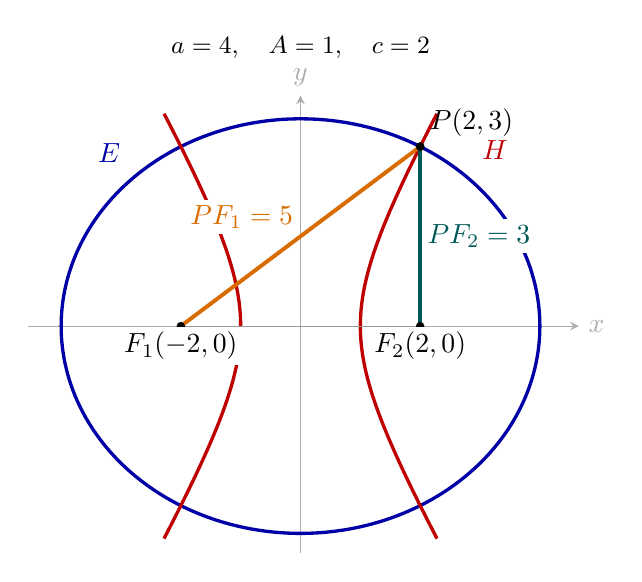
\begin{tikzpicture}[scale=0.76,>=stealth]
 \node[font=\small] at (0,4.65) {$a=4,\quad A=1,\quad c=2$};
 \draw[->,gray!65] (-4.55,0)--(4.65,0) node[right]{$x$};
 \draw[->,gray!65] (0,-3.8)--(0,3.85) node[above]{$y$};
 \draw[blue!65!black,very thick,samples=160,domain=0:360,smooth,variable=\t]
  plot ({4*cos(\t)},{sqrt(12)*sin(\t)});
 \draw[red!75!black,very thick,samples=110,domain=-3.55:3.55,variable=\t]
  plot ({sqrt(1+\t*\t/3)},{\t});
 \draw[red!75!black,very thick,samples=110,domain=-3.55:3.55,variable=\t]
  plot ({-sqrt(1+\t*\t/3)},{\t});
 \coordinate (L) at (-2,0); \coordinate (R) at (2,0); \coordinate (P) at (2,3);
 \draw[orange!85!black,line width=1.4pt] (L)--(P) node[midway,above left,fill=white,inner sep=2pt]{$PF_1=5$};
 \draw[teal!70!black,line width=1.4pt] (R)--(P) node[midway,right,fill=white,inner sep=2pt]{$PF_2=3$};
 \draw[gray!80] (L)--(R);
 \fill (L) circle (2pt) node[below,fill=white,inner sep=2pt]{$F_1(-2,0)$};
 \fill (R) circle (2pt) node[below,fill=white,inner sep=2pt]{$F_2(2,0)$};
 \fill (P) circle (2.1pt) node[above right]{$P(2,3)$};
 \node[blue!65!black] at (-3.2,2.9) {$E$};
 \node[red!75!black] at (3.25,2.95) {$H$};
\end{tikzpicture}

\end{center}

\textbf{识别：}给出两条标准方程，先核查是否共焦，再使用定和、定差。

\textbf{解：}椭圆 $a=4$、$b^2=12$，所以 $c^2=a^2-b^2=16-12=4$；
双曲线 $A=1$、$B^2=3$，所以 $c^2=A^2+B^2=1+3=4$。
两条曲线的焦点确为 $F_1=(-2,0)$、$F_2=(2,0)$。
$P$ 在第一象限，横坐标大于零，属于双曲线右支，所以
\[
\boxed{PF_1=4+1=5,\qquad PF_2=4-1=3}.
\]
\textbf{回验：}$PF_1+PF_2=8=2a$，
$PF_1-PF_2=2=2A$；
这里\emph{无需先求 $P$ 的坐标}。
\end{examplebox}

\clearpage
\begin{examplebox}
\textbf{例2（变式：仅给离心率，并比较左右支）。}

椭圆与双曲线共焦，焦距 $F_1F_2=6$，
椭圆离心率 $e_1=\frac35$，双曲线离心率 $e_2=\frac32$。
$P$ 为第二象限公共点，$Q$ 为第一象限公共点。
分别求 $PF_1,PF_2,QF_1,QF_2$。

\textbf{识别：}给离心率先求半轴；象限直接告诉我们支别。

\textbf{解：}$c=3$，故
\[
a=\frac{3}{3/5}=5,\qquad A=\frac{3}{3/2}=2.
\]
较长的焦半径为 $7$，较短的为 $3$。
$P$ 在左支，离 $F_1$ 较近；$Q$ 在右支，离 $F_2$ 较近。因此
\[
\boxed{PF_1=3,\quad PF_2=7;\qquad QF_1=7,\quad QF_2=3}.
\]
\textbf{回验：}两点的焦半径和都为 $10$，差的绝对值都为 $4$。
\textbf{最小反例：}若给左支点写 $PF_1=7>PF_2=3$，
则与 $PF_1^2-PF_2^2=4cx_P<0$ 矛盾。
\end{examplebox}

\clearpage
\begin{examplebox}
\textbf{例3（反向题：由焦半径还原两条曲线）。}

$F_1=(-4,0)$、$F_2=(4,0)$ 是共焦椭圆与双曲线的焦点。
右支公共点 $P$ 满足 $PF_1=9$、$PF_2=5$。
求椭圆与双曲线的标准方程。

\textbf{识别：}给两条焦半径，反过来使用定和、定差求半轴。

\textbf{解：}由椭圆与双曲线定义，
\[
a=\frac{9+5}{2}=7,\qquad A=\frac{9-5}{2}=2,\qquad c=4.
\]
椭圆半短轴平方 $b^2=a^2-c^2=49-16=33$；
双曲线虚半轴平方 $B^2=c^2-A^2=16-4=12$。
因此
\[
\boxed{E:\ \frac{x^2}{49}+\frac{y^2}{33}=1},\qquad
\boxed{H:\ \frac{x^2}{4}-\frac{y^2}{12}=1}.
\]
\textbf{回验：}$7>4>2>0$，参数满足共焦条件；
$2a=14=9+5$，$2A=4=9-5$。

\textbf{延伸：}若题目要求列出四个公共点及坐标，
可用 C094 的交点坐标方法继续求解，不必在 C093 重做整套推导。
\end{examplebox}
